\documentclass[10pt,landscape]{article}
\usepackage{multicol}
\usepackage{calc}
\usepackage{ifthen}
\usepackage[landscape]{geometry}
\usepackage{hyperref}

\usepackage[OT1]{fontenc}
\usepackage[sc]{mathpazo}
\usepackage[utf8]{inputenc}
\usepackage[german]{babel}
\usepackage{amsmath}
\usepackage{amsfonts}
\usepackage{amssymb}
\usepackage{mathtools}
\usepackage{fancyhdr}
\usepackage{setspace}
\usepackage{listings}
\usepackage{stmaryrd}
\usepackage{graphicx}
\usepackage{changepage}
\usepackage{enumitem}
\usepackage{wrapfig}
\usepackage{tikz} 
\usepackage{xcolor, soul}
\newcommand{\green}[1]{\sethlcolor{green}\hl{#1}}
\newcommand{\yellow}[1]{\sethlcolor{yellow} \hl{#1}}
\newcommand{\blue}[1]{\sethlcolor{cyan} \hl{#1}}


% To make this come out properly in landscape mode, do one of the following
% 1.
%  pdflatex latexsheet.tex
%
% 2.
%  latex latexsheet.tex
%  dvips -P pdf  -t landscape latexsheet.dvi
%  ps2pdf latexsheet.ps


% If you're reading this, be prepared for confusion.  Making this was
% a learning experience for me, and it shows.  Much of the placement
% was hacked in; if you make it better, let me know...


% 2008-04
% Changed page margin code to use the geometry package. Also added code for
% conditional page margins, depending on paper size. Thanks to Uwe Ziegenhagen
% for the suggestions.

% 2006-08
% Made changes based on suggestions from Gene Cooperman. <gene at ccs.neu.edu>


% To Do:
% \listoffigures \listoftables
% \setcounter{secnumdepth}{0}


% This sets page margins to .5 inch if using letter paper, and to 1cm
% if using A4 paper. (This probably isn't strictly necessary.)
% If using another size paper, use default 1cm margins.
\ifthenelse{\lengthtest { \paperwidth = 11in}}
	{ \geometry{top=.5in,left=.5in,right=.5in,bottom=.5in} }
	{\ifthenelse{ \lengthtest{ \paperwidth = 297mm}}
		{\geometry{top=1cm,left=1cm,right=1cm,bottom=1cm} }
		{\geometry{top=1cm,left=1cm,right=1cm,bottom=1cm} }
	}

% Turn off header and footer
\setcounter{page}{1}


% Redefine section commands to use less space
\makeatletter
\renewcommand{\section}{\@startsection{section}{1}{0mm}%
                                {-1ex plus -.5ex minus -.2ex}%
                                {0.5ex plus .2ex}%x
                                {\normalfont\large\bfseries}}
\renewcommand{\subsection}{\@startsection{subsection}{2}{0mm}%
                                {-1explus -.5ex minus -.2ex}%
                                {0.5ex plus .2ex}%
                                {\normalfont\normalsize\bfseries}}
\renewcommand{\subsubsection}{\@startsection{subsubsection}{3}{0mm}%
                                {-1ex plus -.5ex minus -.2ex}%
                                {1ex plus .2ex}%
                                {\normalfont\small\bfseries}}
\makeatother

% Define BibTeX command
\def\BibTeX{{\rm B\kern-.05em{\sc i\kern-.025em b}\kern-.08em
    T\kern-.1667em\lower.7ex\hbox{E}\kern-.125emX}}

% Don't print section numbers
\setcounter{secnumdepth}{0}


\setlength{\parindent}{0pt}
\setlength{\parskip}{0pt plus 0.5ex}


% -----------------------------------------------------------------------

\begin{document}
\raggedright
\footnotesize
\begin{multicols}{3}


% multicol parameters
% These lengths are set only within the two main columns
%\setlength{\columnseprule}{0.25pt}
\setlength{\premulticols}{1pt}
\setlength{\postmulticols}{1pt}
\setlength{\multicolsep}{1pt}
\setlength{\columnsep}{2pt}

\begin{center}
     \Large{\textbf{Compiler Design - Cheatsheet}} \\
\end{center}
\subsection{Simplified Compiler Structure}

\begin{align*}
    &\text{Source Code} \rightarrow \\
    &\underbrace{\text{Lexical Analysis}\rightarrow^{\text{Token Stream}} \text{Parsing}
    \rightarrow^{\text{Abstract Syntax Tree}}}_{\text{Front End}} \\
    &\underbrace{\text{Intermediate Code Generation} \rightarrow^{\text{Intermediate Code}}}_{\text{Middle End}} \\
    &\underbrace{\text{Code Generation}}_{\text{Back End}}
\end{align*}
\subsection{Stack layout}
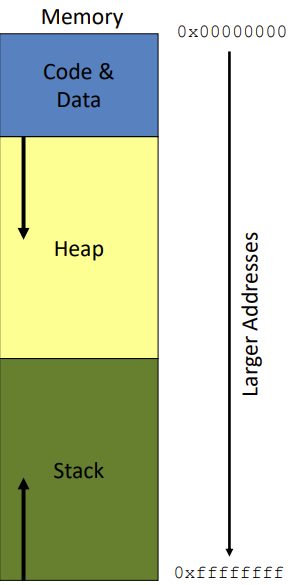
\includegraphics[width = 0.2\textwidth]{Bilder/stack.png}
\subsection{Suffiexes}
\begin{enumerate}
    \item  q = quadword (4 words)
    \item l = long (2 words)
    \item w = word (16-bit)
    \item b = byte (8-bit) 
\end{enumerate}
\subsection{movq-instruction}
movq $SRC$, $DST$ = $DST \leftarrow SRC$ \\
\subsection{Flags}
\begin{center}
    \begin{tabular}{|c|c|} 
     \hline
     e (equality) & ZF is set \\ \hline
     ne (inequality) & (not ZF) \\ \hline
     g (greater than) & (not ZF) and (SF $=$ OF)  \\ \hline
     l (less than) & SF $<>$ OF\\ \hline
     ge (greater or equal) & (SF $=$ OF)  \\ \hline
     le (less than or equal) & SF $<>$ OF or Z  \\ \hline  
    \end{tabular}
  \end{center}
\subsection{Addressing}
\begin{center}
    \begin{tabular}{|c|c|} 
     \hline
     $-8$ ($\%$rsp) & rsp $–$ 8 \\ \hline
     ($\%$rax, $\%$rcx) & rax $+$ 8$\cdot$rcx \\ \hline
     8($\%$rax, $\%$rcx) & rax $+$ 8$\cdot$rcx + 8  \\ \hline
    \end{tabular}
  \end{center}
\subsection{leaq vs. movq}
In leaq we just compute the address, in movq we dereference the address.
\subsection{cmp}
cmpq $SRC1$, $SRC1$ = $SRC2 - SRC1$, flags are set compared to $SRC2$
\subsection{Redzone}
Is an area beyond the current stack frame, scratch pad for the callee's data.\\
%\subsection{Callee vs. Caller saved}
%Caller saved register (Rdi, Rsi, Rdx, Rcx, R09, R08, Rax, R10, R11) are saved by the caller befor calling the function. Callee saved register 
%(Rbx, R12, R13, R14, R15) are saved by the called function. \\
%\subsection{Parameter} 
%\begin{enumerate}
%    \item $1 \dots 6$: rdi, rsi, rdx, rcx, r8, r9
%    \item $7+$: on the stack (in right-to-left order), nth arg. $((n-7)+2) \cdot 8 + rbp$
%\end{enumerate}
%\subsection{Why Intermediate Representations?}
%\begin{enumerate}
%    \item resulting code quality is poor (direct translation)
%    \item Richer source language features are hard to encode (Structured data types, Objects, \dots)
%    \item hard to optimize
%    \item Control-flow is not structured
%\end{enumerate}
%\subsection{Basic Blocks}
%\begin{enumerate}
%    \item Starts with a label that names the entry point of the basic block
%    \item Ends with a control-flow instruction
%    \item Contains no other control-flow instructions
%    \item Contains no interior label used as a jump target
%\end{enumerate}
%\subsection{CFGs}
%\begin{enumerate}
%    \item Nodes are basic blocks
%    \item There is a directed edge from node A to node B if the control flow
%    instruction at the end of block A might jump to the label of block B
%    \item No two blocks have the same label
%\end{enumerate}
\subsection{getelementptr instruction}
The first argument is always a type used as the basis for the calculations. 
The second argument is always a pointer or a vector of pointers, 
and is the base address to start from. The remaining arguments are indices 
that indicate which of the elements of the aggregate object are indexed.
\yellow{GEP never dereferences the address it's calculating}.
%\begin{verbatim}
%struct RT {
%  char A;
%  int B[10][20];
%  char C;
%};
%struct ST {
%  int X;
%  double Y;
%  struct RT Z;
%};
%
%int *foo(struct ST *s) {
%  return &s[1].Z.B[5][13];
%}
%\end{verbatim} 
%is translated in:
%\begin{verbatim}
%    %arrayidx = getelementptr %struct.ST, ptr %s, i64 1, 
%    i32 2, i32 1, i64 5, i64 13
%    ret ptr %arrayidx
%\end{verbatim}
\subsection*{Regular Expressions}
Regular expressions precisely describe sets of strings. A regular expression R has one of the following forms:
\begin{enumerate}
  \item $\epsilon$: Epsilon stands for the empty string
  \item $'a'$: An ordinary character stands for itself
  \item $R_1 | R_2$: Alternatives, stands for choice of $R_1$ or $R_2$
  \item $R_1 R_2$: Concatenation, stands for $R_1$ followed by $R_2$
  \item $R^*$: Kleene star, stands for zero or more repetitions of $R$
\end{enumerate}
Useful extensions:
\begin{enumerate}
  \item "$foo$": Strings, equivalent to $'f'$ $'o'$ $'o'$
  \item $R^+$: One or more repetitions of $R$, equivalent to $RR^*$
  \item $R$?: Zero or one occurrences of $R$, equivalent to $(\epsilon|R)$
  \item $['a'-'z']$: One of $a$ or $b$ or $c$ or \dots $z$, equivalent to $(a|b|\dots|z)$
  \item $[\text{ }\Hat{ }\text{  }'0'-'9']$: Any character except $0$ through $9$
  \item $R$ as $x$: Name the string matched by $R$ as $x$
\end{enumerate}
\subsection{Chomsky Hierarchy}
Regular $\subset$ Context-Free $\subset$ Context Sensitive $\subset$ Recursively Enumerable \\
\subsection{Matching Rule for Lexer}
Most languages choose “longest match”.
\subsection{Lexer Generator}
\begin{enumerate}
  \item Reads a list of regular expressions: $R_1,\dots,R_n$ , one per token
  \item Each token has an attached “action” $A_i$ (just a piece of code to run
  when the regular expression is matched)  
\end{enumerate}
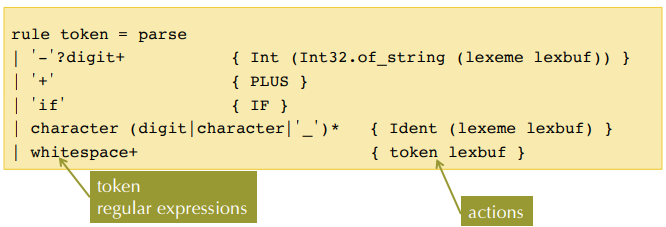
\includegraphics[width = 0.3\textwidth]{Bilder/lexer_generator.png}
Generates scanning code that:
\begin{enumerate}
  \item Decides whether the input is of the form $(R_1|\dots|R_n)^*$
  \item After matching a (longest) token, runs the associated action 
\end{enumerate}
\subsection{Implementation Strategies}
We can use a finite automaton since one must exist for a regular expression.
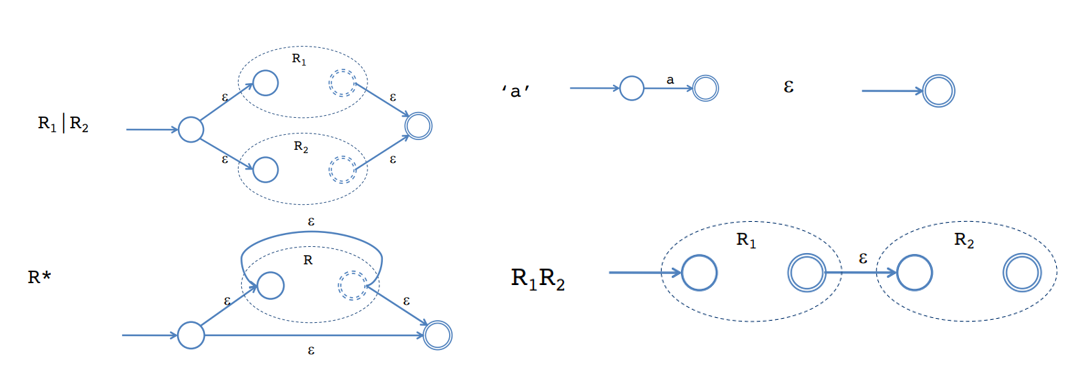
\includegraphics[width = 0.3\textwidth]{Bilder/nfas.png}
\subsection{DFA vs. NFA}
DFA:
\begin{enumerate}
  \item Action of the automaton for each input is fully determined
  \item Accepts if the input is consumed upon reaching an accepting state
  \item Obvious table-based implementation
\end{enumerate}
NFA:
\begin{enumerate}
  \item Automaton potentially has a choice at every step
  \item Accepts an input if there exists a way to reach an accepting state
  \item Less obvious how to implement efficiently
\end{enumerate}
\subsection{Parsing}
\textbf{Def.:} Finding Syntactic Structure \\
\textbf{Limits of regular expressions}:
\begin{enumerate}
  \item DFA's have only finite \# of states (i.e., finite memory)
  \item So, DFA's can't count
\end{enumerate}
Therefore we need something more powerful than DFA's.
\subsection{CONTEXT FREE GRAMMARS}
\textbf{Def. recursive:} $S$ mentions itself, e.g. $S \mapsto (S)S$
A Context-free Grammar (CFG) consists of 
\begin{enumerate}
  \item A set of terminals (e.g., a lexical token, $\epsilon$ is not a terminal)
  \item A set of nonterminals (e.g., S and other syntactic variables)
  \item A designated nonterminal called the start symbol
  \item A set of productions: $LHS \mapsto RHS$
\end{enumerate}
\textbf{single step:} For arbitrary strings $\alpha, \beta, \gamma$ and production rule $A \mapsto \beta$ a single step of the derivation is
$\alpha A \gamma \mapsto \alpha \beta \gamma$ \\
\textbf{ Parse Tree:} Leaves are terminals and Internal nodes are nonterminals.\\
%\subsection{Parse Trees to Abstract Syntax}
%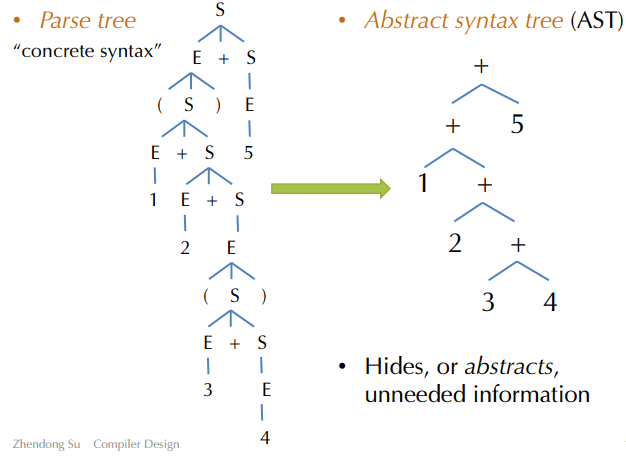
\includegraphics[width = 0.3\textwidth]{Bilder/parse_tree_ast.png}
\subsection{Derivation Orders}
Productions of the grammar can be applied in any order. Both strategies (and any other) yield the \yellow{same} parse tree!
\begin{enumerate}
  \item Leftmost derivation: Find the left-most nonterminal and apply a production to it e.g. $S \mapsto \underline{\textbf{E}} + S$
  \item Rightmost derivation: Find the right-most nonterminal and apply a production there e.g. $S \mapsto E + \underline{\textbf{S}}$
\end{enumerate}
\textbf{productive and nonproductive:} This grammar has nonterminal definitions that don't mention any terminal symbols.\\
\textbf{finite:} There is a finite derivation starting from start symbol.\\
\textbf{Example of right associative:} $S \mapsto E + S | E$, $E \mapsto \text{number} | ( S )$ \\
\textbf{Example of Ambiguity:} $S \mapsto S + S | ( S ) | \text{number}$, accepts the same set of strings as the previous one
but there are two leftmost derivations. Moreover, if there are multiple operations, ambiguity in the grammar
leads to ambiguity in their precedence.\\
\textbf{Eliminating Ambiguity:} 
\begin{enumerate}
  \item by adding nonterminals and allowing recursion only on the left (or right)
  \item Higher-precedence operators go farther from the start symbol
\end{enumerate}
\textbf{Example of Eliminating Ambiguity:} $S \mapsto S + S | ( S ) | \text{number}$ becomes $S_0 \mapsto S_0 + S_1 | S_1$, 
$S_1 \mapsto S_2 * S_1 | S_2$ and $S_2 \mapsto \text{number} | ( S_0 )$
\subsection{LL(1) GRAMMARS}
\textbf{Top-down:} Start from the start symbol (root of the parse tree), and go down. Not all grammars can be parsed "top-down" with a single lookahead. \\
LL(1) means:
\begin{enumerate}
  \item \textbf{L}eft-to-right scanning
  \item \textbf{L}eft-most derivation
  \item \textbf{1} lookahead symbol
\end{enumerate}
\subsection{Making a grammar LL(1)}
\textbf{Problem:} We can't decide which $S$ production to apply until we see the symbol after the first expression
\textbf{Solution:} “Left-factor” the grammar. There is a common $S$ prefix for each choice, so add a new non-terminal $S'$ at the decision point.
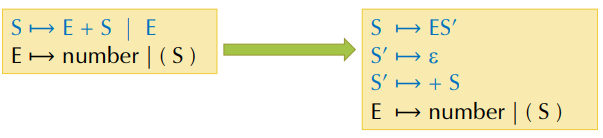
\includegraphics[width = 0.2\textwidth]{Bilder/left_factor.png}\\
Also need to eliminate left-recursion.
$\mathrm{S} \mapsto \mathrm{S} \alpha_1|\ldots| \mathrm{S} \alpha_n\left|\beta_1\right| \ldots \mid \beta_{\mathrm{m}}$ becomes
$\mathrm{S} \mapsto \beta_1 S^{\prime}|\ldots| \beta_{\mathrm{m}} S^{\prime}$
$S^{\prime} \mapsto \alpha_1 S^{\prime}|\ldots| \alpha_n S^{\prime} \mid \varepsilon$\\
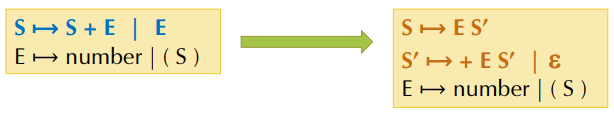
\includegraphics[width = 0.2\textwidth]{Bilder/elemination_left_rec.png}
\subsection{Predictive Parsing}
For a given nonterminal, the lookahead symbol uniquely determines the production to apply. Therefore we get a table 
with $\text{nonterminal} \times \text{input token} \rightarrow \text{production}$
\subsection{Construction of the parse table:}
Consider a given production: $A \mapsto \gamma$. 
\begin{enumerate}
  \item (Case 1) Construct the set of all input tokens that may appear first in strings that can be derived from $\gamma$.
  Add the production $\mapsto \gamma$ to the entry $(A,\text{token})$ for each such token.
  \item (Case 2) If $\gamma$ can derive $\epsilon$ (the empty string), then we construct the set of all input tokens that may follow the nonterminal $A$ in the grammar.
  Add the production $\mapsto \gamma$ to the entry $(A,\text{token})$ for each such token.
\end{enumerate}
\textbf{Example: }
We have $T \mapsto S\$, S \mapsto ES', S' \mapsto e, S' \mapsto + S, E \mapsto \text{number} | ( S )$. We get
\begin{enumerate}
  \item First(S\$) = First(S) = First(E') = First(E) = \{ number, '(' \}
  \item First($\epsilon$) = \{ $\epsilon$ \}
  \item First($+$S) = \{ $+$ \}
  \item First(number) = \{ number \}
  \item First( (S) ) = \{ '(' \}
  \item Follow(S') = Follow(S)
  \item Follow(S) = \{ \$, ')' \} $\cup$ Follow(S')
\end{enumerate}
\subsection{LR GRAMMARS}
LR(k) parser
\begin{enumerate}
  \item Bottom-up Parsing
  \item \textbf{L}eft-to-right scanning
  \item \textbf{R}ightmost derivation
  \item \textbf{k} lookahead symbols
\end{enumerate}
LR grammars are more expressive than LL. Can handle left-recursive (and right recursive) grammars.
\subsection{Shift/Reduce Parsing}
\textbf{Shift:} Move look-ahead token to the stack \\
\textbf{Reduce:}: Replace symbols $\gamma$ at top of stack with nonterminal $X$ s.t. $X \mapsto \gamma$ is a production
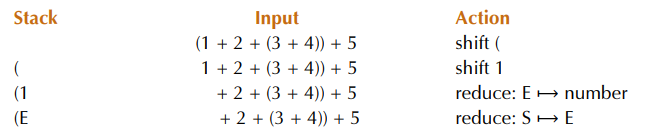
\includegraphics[width = 0.3\textwidth]{Bilder/shift_reduce.png}
\textbf{LR(0) state:} items to track progress on possible upcoming reductions\\
\textbf{LR(0) item:}  a production with an extra separator "." in the RHS, e.g. $S \mapsto .(L)$ or $S \mapsto (.L)$. Idea is
stuff before the '.' is already on the stack and stuff after the '.' is what might be seen next. 
\subsection{Constructing the DFA: Start state \& Closure}
\begin{enumerate}
  \item Start state of the DFA = empty stack, so it contains the item $S' \mapsto .S\$$
  \item Closure of a state: Adds items for all productions whose LHS nonterminal occurs in an item in the state 
  just after the '.' (e.g., $S$ in $S' \mapsto .S\$$). The added items have the '.' located at the beginning (no symbols for
  those items have been added to the stack yet), e.g. CLOSURE$(\{S' \mapsto .S\$\}) = \{S' \mapsto .S\$, S \mapsto .(L), S \mapsto .\text{id}\}$
  \item Next we add the transitions, e.g after reading id we get $S \mapsto \text{id}.$
  \item Finally, for each new state, we take the closure
  \item If a reduce state is reached, reduce otherwise, if the next token matches an outgoing edge, shift
\end{enumerate}
\subsection{Implementing the Parsing Table}
Entries for the “action table” specify two kinds of actions: Shift and go to state n and Reduce using reduction $X \mapsto \gamma$.
We only have reduction when we don't have any outgoing edges otherwise we shift.
\subsection{LR(0) Limitations}
\textbf{shift/reduce:} $S \mapsto (L).$ and $L \mapsto .L, S$ yield a problem in a state since with $(L).$ we are allowed to reduce
but with $.L$ we are also allowed to shift.
\textbf{ reduce/reduce:} $S \mapsto L, S.$ and $S \mapsto ,S.$ yield a problem in a state since there exists two diffrent
reduction rules for $S.$
\subsection{LR(1) Parsing}
\begin{enumerate}
  \item LR(1) state = set of LR(1) items
  \item An LR(1) item is an LR(0) item + a set of look-ahead symbols $A \mapsto \alpha.\beta, \mathcal{L}$
\end{enumerate}
\textbf{LR(1) closure:}
\begin{enumerate}
  \item Form the set of items just as for LR(0) algorithm
  \item Whenever a new item $C \mapsto .\gamma$ is added because $A \mapsto \beta.C\delta, \mathcal{L}$ is
  already in the set, we need to compute its look-ahead set $\mathcal{M}$ 
  \begin{enumerate}
    \item The look-ahead set $\mathcal{M}$  includes FIRST($\delta$) 
    \item If $\delta$ is or can derive $\epsilon$, then the look-ahead $\mathcal{M}$ also contains $\mathcal{L}$
  \end{enumerate} 
\end{enumerate}
\textbf{Example Closure:} Asume we have $S' \mapsto S\$, S \mapsto E + S | E, E \mapsto \text{number}|S$
\begin{itemize}
  \item Start item: $S' \mapsto S\$, \{\}$
  \item Since $S$ is to the right of a '.', add $S \mapsto .E + S, \{\$\}; S \mapsto .E, \{\$\}$
  \item Need to keep closing, since $E$ appears to the right of a '.' in '.E + S', $E \mapsto .\text{number}, \{+\}; E \mapsto .(S), \{+\}$
  \item Because E also appears to the right of . in .E we get: $E \mapsto .\text{number}, \{\$\}; E \mapsto .(S), \{\$\}$
  \item All items are distinct, so we’re done
\end{itemize}
\textbf{Ambiguity with if else:} \begin{verbatim}
  if (E1) if (E2) S1 else S2
\end{verbatim}
This is known as the \yellow{dangling else problem}. What should the right answer be?
We know two solutions: the simple one would just require \{\} and another one could use the grammar
\begin{enumerate}
  \item $S \mapsto M | U$   // M = matched, U = unmatched
  \item $U \mapsto$ if (E) S   // Unmatched if
  \item $U \mapsto$ if (E) M else U  // Nested if is matched
  \item $M \mapsto$ if (E) M else M // Matched if
  \item $M \mapsto$ X = E  // Other statements
\end{enumerate}
\subsection{Lambda Calculus}
The lambda calculus is a minimal programming language. It has variables, functions, and function application.
It's Turing Complete. Concrete syntax:
\begin{verbatim}
  exp ::=
      | x               //variables
      | fun x -> exp    //functions
      | exp1 exp2       //function application
      | ( exp )         //parentheses
\end{verbatim}
The only values of the lambda calculus are (closed) functions that is val ::= fun x $\rightarrow$ exp.\\
\textbf{substitute:} Replace all free occurrences of $x$ in $e$ by $v$ also written as $e\{v/\}$ If we try to substitute a
variable which is not free, the expression remains the same.\\
$\mathrm{x}\{\mathrm{v} / \mathrm{x}\} \quad=\mathrm{v} \quad$ (replace the free $x$ by $v$ )\\
$y\{v / x\} \quad=y \quad$ (assuming $y \neq x$ )\\
$($ fun $x\rightarrow\exp )\{v / x\} \quad=($ fun $x \rightarrow \exp ) \quad$ ( $x$ is bound in exp)\\
$($ fun $y\rightarrow\exp )\{v / x\} \quad=($ fun $y\rightarrow \exp \{v / x\}) \quad$ (assuming $y \neq x$ )\\
$\left(\mathrm{e}_1 \mathrm{e}_2\right)\{\mathrm{v} / \mathrm{x}\} \quad=\left(\mathrm{e}_1\{\mathrm{v} / \mathrm{x}\} \mathrm{e}_2\{\mathrm{v} / \mathrm{x}\}\right) \quad$ (substitute everywhere)\\
\textbf{free variable:} We say variable x is free in fun y $\rightarrow$ x + y. Free variables are defined in an outer scope\\
\textbf{bound variable:} We say variable y is bound by fun y. Its scope is the body x + y in fun y $\rightarrow$ x + y\\
\textbf{closed:} A term with no free variables is called closed. \\
\textbf{open:} A term with one or more free variables is called open.
\textbf{Free Variable Calculation:}\\
$fv(x) = \{x\}$ \\
$fv(\operatorname{fun} x \rightarrow \exp) = fv(\exp) \backslash \{x\}$ \\
$fv(\exp_1 \exp_2) = fv(\exp_1) \cup fv(\exp_2)$\\
\textbf{Variable Capture:} In $(\operatorname{fun} x \rightarrow (x y)) \{(\operatorname{fun} z \rightarrow x) / y\} = \operatorname{fun} x \rightarrow (x (\operatorname{fun} z \rightarrow x))$
$x$ is captured. Usually not the desired behavior. This property is sometimes called dynamic scoping. The meaning of $x$ is determined by where it is bound
dynamically. \\
\textbf{Alpha Equivalence:} Two terms that differ only by consistent renaming of bound variables are called alpha equivalent, e.g. $(\operatorname{fun} x \rightarrow y x)$ the same as $(\operatorname{fun} z \rightarrow y z)$\\
\subsection{Operational Semantics}
$\frac{}{v \Downarrow v}$ \\
$\frac{\exp _1 \Downarrow\left(\text { fun } x\rightarrow \exp _3\right) \quad \exp _2 \Downarrow v \quad \exp _3\{v / x\} \Downarrow w}{\exp _1 \exp _2 \Downarrow w}$
\subsection{Y Combinator \& Factorial}
\textbf{Y combinator:} $Y = = \backslash f. (\backslash x. f (x\text{ }x)) (\backslash x. f (x \text{ }x))$. Y F = F (Y F) for any term F.
\textbf{Example factorial function:}
\begin{itemize}
  \item Typical recursive definition: $fac = \backslash n. if (n=0) 1 (n * fac (n-1))$
  \item Abstract it: $F = \backslash f. \backslash n. if (n=0) 1 (n * f(n-1))$
  \item Thus, fac = F fac (i.e., fac is a fixpoint of F)
  \item Y F being fixpoint of F can thus be viewed as the factorial function!
\end{itemize}
\subsection{CLOSURE CONVERSION}
The closure is a pair of the environment and a code pointer: Code(env, y, body). We get 
fun (env, y) $\rightarrow$ let x = nth env 0 in body, where y is possibly in body.\\
\textbf{Array-based Closures with N-ary Functions:} 
We have (fun (x y z) $\rightarrow$ (fun (n m) $\rightarrow$ (fun p $\rightarrow$ (fun q $\rightarrow$ n + z) x)))
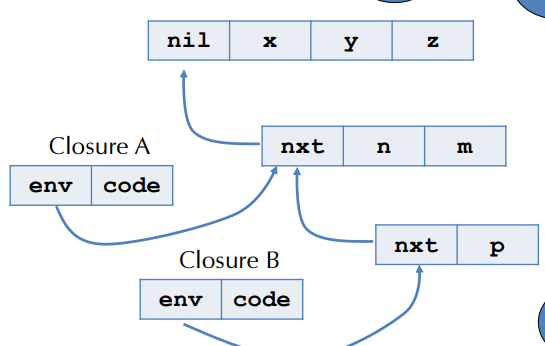
\includegraphics[width = 0.2\textwidth]{Bilder/closure_array_based.png}\\
\textbf{Theorem: (simply typed lambda calculus with integers):} If $\vdash e : t$, then there exists a value $v$ such that $e \Downarrow v$ \\
\textbf{Theorem: (Type Safety)} If $\vdash P : t$ is a well-typed program, then either
\begin{enumerate}
  \item the program terminates in a well-defined way, or
  \item the program continues computing forever
\end{enumerate}
\textbf{type:} A type is just a predicate on the set of values in a system. E.g., the type int can be thought of as a boolean function that returns
true on integers and false otherwise. Equivalently, we can think of a type as just a subset of all values.\\
\textbf{subtype:} This subset relation gives rise to a subtype relation: if $Pos <: Int$, then Pos is a subtype of Int \\
\textbf{LUB:} least upper bound, for statically unknown conditionals, we want the return value to be
the LUB of the types of the branches. LUB is also called the join operation. \\
subtyping relation is a \textbf{partial order}, that is:
\begin{enumerate}
  \item Reflexive: T <: T for any type T
  \item Transitive: T1 <: T2 and T2 <: T3 then T1 <: T3
  \item Antisymmetric: It T1 <: T2 and T2 <: T1 then T1 = T2
\end{enumerate}
\textbf{Soundness of Subtyping Relations:} A subtyping relation T1 <: T2 is sound if it approximates the underlying
semantic subset relation, that is let be $\llbracket T \rrbracket=\{v \mid \vdash v: T\}$. If T1 <: T2 implies $\llbracket T1 \rrbracket \subseteq  \llbracket T2 \rrbracket$, then T1 <: T2 is sound.
Whenever we have a sound subtyping relation, it follows that $\llbracket L U B\left(\mathrm{~T}_1, \mathrm{~T}_2\right) \rrbracket \supseteq \llbracket \mathrm{T}_1 \rrbracket \cup \llbracket \mathrm{T}_2 \rrbracket$.
Using LUBs in the typing rules yields sound approximations of the program behavior (as if the IF-B rule)\\
\textbf{Subsumption Rule:} $\frac{E \vdash e : T \quad  T <:  S}{E \vdash e : S}$\\
\textbf{Subtyping for Function Types:} Need to convert an S1 to a T1 and T2 to S2, so the argument type is
contravariant and the output type is covariant: $\frac{S1 <: T1 \quad T2 <: S2}{(T1 \rightarrow T2) <: (S1 \rightarrow S2)}$\\
\textbf{reference types:} Are not covariant because of 
\begin{verbatim}
  Int bad(NonZero ref r) {
    Int ref a = r; (* OK because NonZero ref <: Int ref *)
    a := 0; (* OK because 0 : Zero <: Int *)
    return (42 / !r) (* OK because !r has type NonZero *)
  }
\end{verbatim}
and not contravariant because of 
\begin{verbatim}
  Assume: NonZero <: Int => ref Int <: ref NonZero
  Int ref a;
  a := 0;
  NonZero ref b;
  b = a;
  return (1 / !b); 
\end{verbatim}
\textbf{Immutable Record Subtyping:} it holds $\{x:int, y :int\} \neq \{y:int, x:int\}$ and $\{x:int, y :int, z:int\} <: \{x:int, y :int\}$\\
\textbf{Mutable Structures:} Mutable structures are invariant that is $T_1 ref <: T_2 ref \Longrightarrow T_1 = T_2$\\
\textbf{Structural vs. Nominal Typing:} Checking against the name is nominal typing and checking against the structure is structural typing.
\subsection{Compiling Objects}
Objects contain a pointer to a dispatch vector (also called a virtual table or vtable) with pointers to method code \\
\textbf{Single Inheritance:} every method has its own small integer index, Index is used to look up the method in the dispatch vector. Each interface and class gives rise to a dispatch vector layout. DV layout of new method is appended to the class which is being extended\\
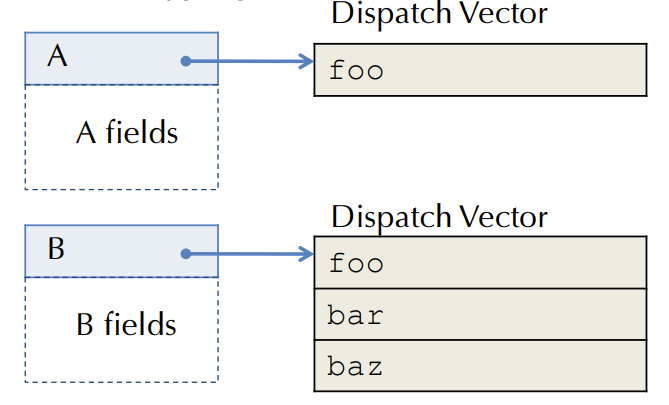
\includegraphics[width = 0.2\textwidth]{Bilder/dv_layout.png}\\
\textbf{Multiple Inheritance:} Multiple Inheritance approaches: Allow multiple DV tables (C++) Choose which DV to use based on 
static types, casting requires runtime operations; Use a level of indirection: Map method identifiers to code pointers 
using a hash table, search up through the class hierarchy; Give up separate compilation: Now we have access to the whole class hierarchy. Use sparse dispatch vectors or 
binary decision trees.
\subsection{Optimization}
An optimization must always be safe i.e. it must not change the behavior of the program.
\begin{itemize}
	\item Problem: many optimizations trade space for time (e.g. Loop unrolling)
	\item Constant Folding: If operands are statically known, compute value at compile-time (has to preformed at every stage of optimization - constant expressions can be created by translation or earlier optimizations / can enable further optimizations). Also: Algebraic Simplification (Use mathematical identities e.g $a \cdot 1 \rightarrow a$)
	\item Copy Propagation: For x = y replace uses of x with y
	\item Dead Code Elimination: If side-effect free code can never be observed, safe to eliminate it
	\item Inlining: Replace a function call with the body of the function (arguments are rewritten)
	\item Code Specialization: Create Specialized versions of a function that is called form different places with different arguments.
	\item Common Subexpression Elimination: In some sense, it is the opposite of inlining: fold redundant computations together
	\item Loop Optimizations
	\begin{itemize}
		\item Hot spots often occur in loops (esp. inner loops)
		\item Loop Invariant Code Motion
		\item Strength Reduction (replace expensive ops by cheap ones by creating a dependent induction variable)
		\item Loop unrolling
	\end{itemize}
\end{itemize}
\subsection{Code Analysis}
Algorithm for Dataflow Analysis:
\begin{verbatim}
  let w = new set with all nodes
  repeat until w is empty
    let n = w.pop()
    old_out = out[n]
    let in = combine(preds[n])
    out[n] := flow[n](in)
    if (!equal old_out out[n]),
      for all m in succs[n], w.add(m)
end
\end{verbatim}
\begin{itemize}
	\item Liveness
	\begin{itemize}
		\item Observation: uid1 and uid2 can be assigned to the same register if their values will not be needed at the same time. Liveness property is more fine grained than scope.
		\item Variable v is live at a program point L if v is defined before L and v is used after L
		\item Liveness analysis is one example of dataflow analysis: A variable $v$ is live on edge $e$ if there is a node n in the CFG such that use[n] contains $v$ and a directed path from e to n such that for every statement $s'$ on the path def[$s'$] does not contain $v$
		\item Dataflow: Compute information for all variables simultaneously. Solve the equations by iteratively converging on a solution: Start with a rough approximation to the answer, refine the answer at each iteration, keep going until nor more refinement is possible.
		\end{itemize}
		\end{itemize}
	  \textbf{Liveness:} backward, may $(out[n] = \bigcup_{n' \in succ[n]} in[n'], in[n] = gen[n] \cup (out[n] \setminus kill[n])), gen[n] = use[n], kill[n] = def[n]$\\
		\textbf{Reaching Definition:} (for Constant and Copy propagation)forward, may $(in[n] = \bigcup_{n' \in pred[n]} out[n'], out[n] = gen[n] \cup (out[n] \setminus kill[n])), gen[n] = \{n\}, kill[n] = defs[a]\setminus \{n\}$\\
		\textbf{Available Expressions:} forward (replace expression with res e.g. a = x + 1, b = x + 1 $\rightarrow$ b = a), must $(in[n] = \bigcap_{n' \in pred[n]} out[n'], out[n] = gen[n] \cup (out[n] \setminus kill[n])), gen[n] = \{n\} \setminus kill[n], kill[n] = uses[a]$\\
    \textbf{Very Busy Expressions:} Expression e is very busy at location p if every path from p
    must evaluate e before any variable in e is redefined, background, must $(out[n] = \bigcap_{n' \in pred[n]} out[n'], in = gen union (out \setminus kill))$\\
		Key idea: Iterative solution of a system of equations over a lattice. Iteration terminates if flow functions are monotonic, equivalent to the MOP answer if flow functions distribute over meet
\subsection{Register Allocation}
\textbf{Linear-Scan Register:} Compute liveness information for each temp, try to use a reg if not possible than spill
\begin{itemize}
	\item Register Allocation: Compute liveness information for each temp, create an infereence graph, try to color the graph.
	\item Kempe: 1. Find a node with degree < k and cut it out of the graph, 2. Recursively k-color the remaining subgraph, 3. When remaining graph is colored, there must be at least one free color available for the deleted node. If the graph cannot be colored we spill that node.
	\item Precolored nodes: Certain variables must be pre-assigned to registers (call, imul, caller-save registers)
\end{itemize}
\textbf{Coalescing Interference Graphs:} A more aggressive strategy is to coalesce nodes of the interference
graph if they are connected by move-related edges (if t1 and t2 in movq t1, t2 can be assigned the same register (color)) this move is
redundant and can be eliminated\\
\textbf{Brigg's strategy:} It's safe to coalesce x \& y if the resulting node will have fewer than k neighbors that have degree >= k. \\
\textbf{George's strategy:} We can safely coalesce x \& y if for every neighbor t of x, either t already interferes with y or t has degree < k.
\subsection{Loops}
Identify loops \& nesting structure in a CFG
\begin{itemize}
	\item A loop is a strongly connected component (head reachable from each node)
	\item Concept of dominators: A dominates B = if the only way to reach B from start node is via A. A loop contains at least 1 back edge. (back edge = target dominates the source), for strictly dominance it must also hold $A \neq B$.
	\item dom is transitive and anti-symmetric, can be computed as a forward dataflow analysis $in[n] = \bigcap_{n' \in pred[n]}out[n'], out[n] = in[n] \cup \{n\}, \bigsqcap = \cap$
\end{itemize}
\subsection{Single Static Assignment (SSA)}
\begin{itemize}
  \item \%uids on RHS of phi nodes can be defined “later” in CFG
  \item An alloca inst. is promotable if the address of the variable is not taken or is not passed by reference
  \item $\phi$ nodes can be placed at dominator tree join nodes (There where $J[N] = DF_i[N] = DF_{i + 1}[N]$ (fixpoint) with $DF_{i + 1}[N] = DF[N \cup DF_i[N]]$ and $N$ as a set of nodes which modify the variable)
	\item eliminate phi nodes after optmization
\end{itemize}
\subsection{dominance frontier}
$DF[X] = \{y | \exists M \rightarrow y \land (X \text{ dom } M) \land \lnot (X \text{ sdom } y) \}$
%Algorithm For Computing Dominance Frontiers:
%\begin{verbatim}
%  for all nodes B
%    if #(pred[B]) >= 2             // (just an optimization)
%      for each p in pred[B] {
%        runner := p        // start at the predecessor of B
%        while (runner != doms[B])  // walk up the tree adding B
%          DF[runner] := DF[runner] union {B}
%          runner := doms[runner]
%      }
%\end{verbatim}
\subsection{Garbage Collector}
\begin{itemize}
	\item Garbage: An object x is reachable iff a register contains a pointer to x or another reachable object y contains a pointer to x
	\item reachable objects can be found by starting from registers and following all pointers
  \item Mark and Sweep
	
	When memory runs out, GC executes two phases: mark phase: trace reachable objects; sweep phase: collects garbage objects (extra bit reserved for memory management)
	
	Pointer reversal enables a depth first traversal of the reachable objects without using additional memory. It maintains the “stack” in the objects themselves by storing pointers that
  point back to their parents in already available memory. 
	\item Stop and Copy
	
	Memory is organized into two areas: Old space (used for allocation), new space (use as a reserve for GC)
	
	When old space is full all reachable objects are moved, old and new are swapped.
  Stop and Copy moves objects around. Pointers to those objects must also be updated.
However, objects (structs) in C and C++ do not carry any metadata that identify which
members are pointers and therefore it is impossible to properly update them. Even if the
garbage collector had access to such information, a pointer can be converted to an integer
and back, the collector cannot know the programmer’s intention and whether it should also
update such integers.
	\item Reference Counting
	
	Store number of references in the object itself, assignments modify that number. Cannot collect circular structures, since each cyclic structure member’s reference count can never drop below 1 (since another
  member of the cycle points to it) even if none of them is reachable.
	For each assignment, $x = y$ The reference count of y's pointer is increased by 1 and that one of x's pointer is decreased by 1.

\end{itemize}
\newpage
\end{multicols}
\end{document}
